Both the original study by Shu et al.~\cite{shu2021predicting} and the subsequent replication and reproducibility study by 
Arafe et al.~\cite{Arafe2023.05.05.539590} selected patients with Parkinson's disease (PD) from the PPMI dataset and matched their 
age, sex, and H\&Y score from the first of two visits spanning approximately 36 months apart. For the first visit, each patient 
underwent an evaluation consisting of a clinical assessment and an MRI scan. They also had a follow-up clinical examination 3 years later. 
Patients were classified as 'progressive' if their H\&Y score at the follow-up visit exceeded the score from 3 years prior; otherwise, they 
were classified as 'stable'. Regarding inclusion criteria, Shu et al. created a cohort by limiting their selection to patients with MRI data 
from a Siemens Verio 3T MRI machine, incorporating restrictions on repetition time, echo time, inversion time, field of view, matrix size, 
and slice thickness. Their final cohort comprised 144 patients, equally distributed between progressive and stable subjects. 
On the other hand, rather than a single cohort, Arafe et al. constructed 5 cohorts, each consisting of 72 stable and 72 progressive subjects. One 
cohort aimed to replicate the Shu et al. cohort, while the other four were designed with different levels to assess the sensitivity of model predictions to 
the selection process.

Like Arafe et al. and Shu et al., as part of the selection process, we filtered the subjects in the PPMI database using the 
following inclusion criteria:
\begin{itemize}
  \item \textbf{C1}: patient has a diagnosis of idiopathic PD;
  \item \textbf{C2}: PPMI database contains records of at least 2 visits spaced approximately 3 years apart;
  \item \textbf{C3}: PPMI database contains a T1-weighted MRI from the first visit determined by C2;
  \item \textbf{C4}: PPMI database contains H\&Y scores for both visits. 
\end{itemize}

We assessed the impact of the MRI machine manufacturers and models on the collected image data and concluded that restrictions on these parameters could be relaxed. 
However, we ensured consistency across the selected subjects by standardizing the slice thickness and field strength across all MRI machines used. Consequently, our 7 
cohorts have been established according to the following additional criteria:

\begin{itemize}
  \item \textbf{C5}: all MRI machine manufacturers and models are permissable;
  \item \textbf{C6}: scanner restrictions: slice thickness = 1 mm and field strength = 3T;
\end{itemize}

After filtering the PPMI dataset for Criteria 1 to 6, visit pairs were formed for the remaining subjects while ensuring C2 and C3 remained true for each visit pair. 
During this phase, an additional restriction was imposed for the formation of Cohorts 1 to 6 such that a patient's functional state (also called PD state), which 
may be ``On" or ``Off", must be the same for both visits. The functional state of a patient, ``On" or ``Off", is determined by their PD medication status during clinical 
examinations. As the classification into progressive or stable groups depends on the stability of H\&Y scores over time, this restriction bolsters the comparability of 
these scores.

As the PPMI dataset is collected over an extended period of time and the protocol requires clinical evaluation in both ``On" and ``Off" functional states for every visit, many 
subjects have more than one visit pair and it is possible for a subject to be classified as both progressive and stable for different visit pairs. Therefore, after the 
creation of a cohort, validation checks were defined to ensure that any given subject was only included once, as either stable or progressive, in the resulting cohort. 

One of our objectives was to create the largest possible cohorts that adhered to the stated restrictions. Thus, although Cohorts 1, 3, 5, and 7 were created 
by matching patients from the progressive and stable classes on age, sex and H\&Y scores from the first visit, Cohorts 2, 4, and 6 used no matching filter.
This approach allowed for larger cohorts but necessitated the creation of demographics feature sets to evaluate the impact of this uneven distribution on the results. 
Cohorts 1 and 2 sampled visit pairs with PD state = "Off", Cohorts 5 and 6 sampled pairs with PD state = "On", and Cohorts 3 and 4 sampled visit pairs with 
either PD state = "Off" or PD state = "On" for both visits. Cohort 7 was defined without any restrictions on the PD state (see Fig~\ref{cohortCreationFlowchart}).

\begin{figure}[!ht]
  \centering
  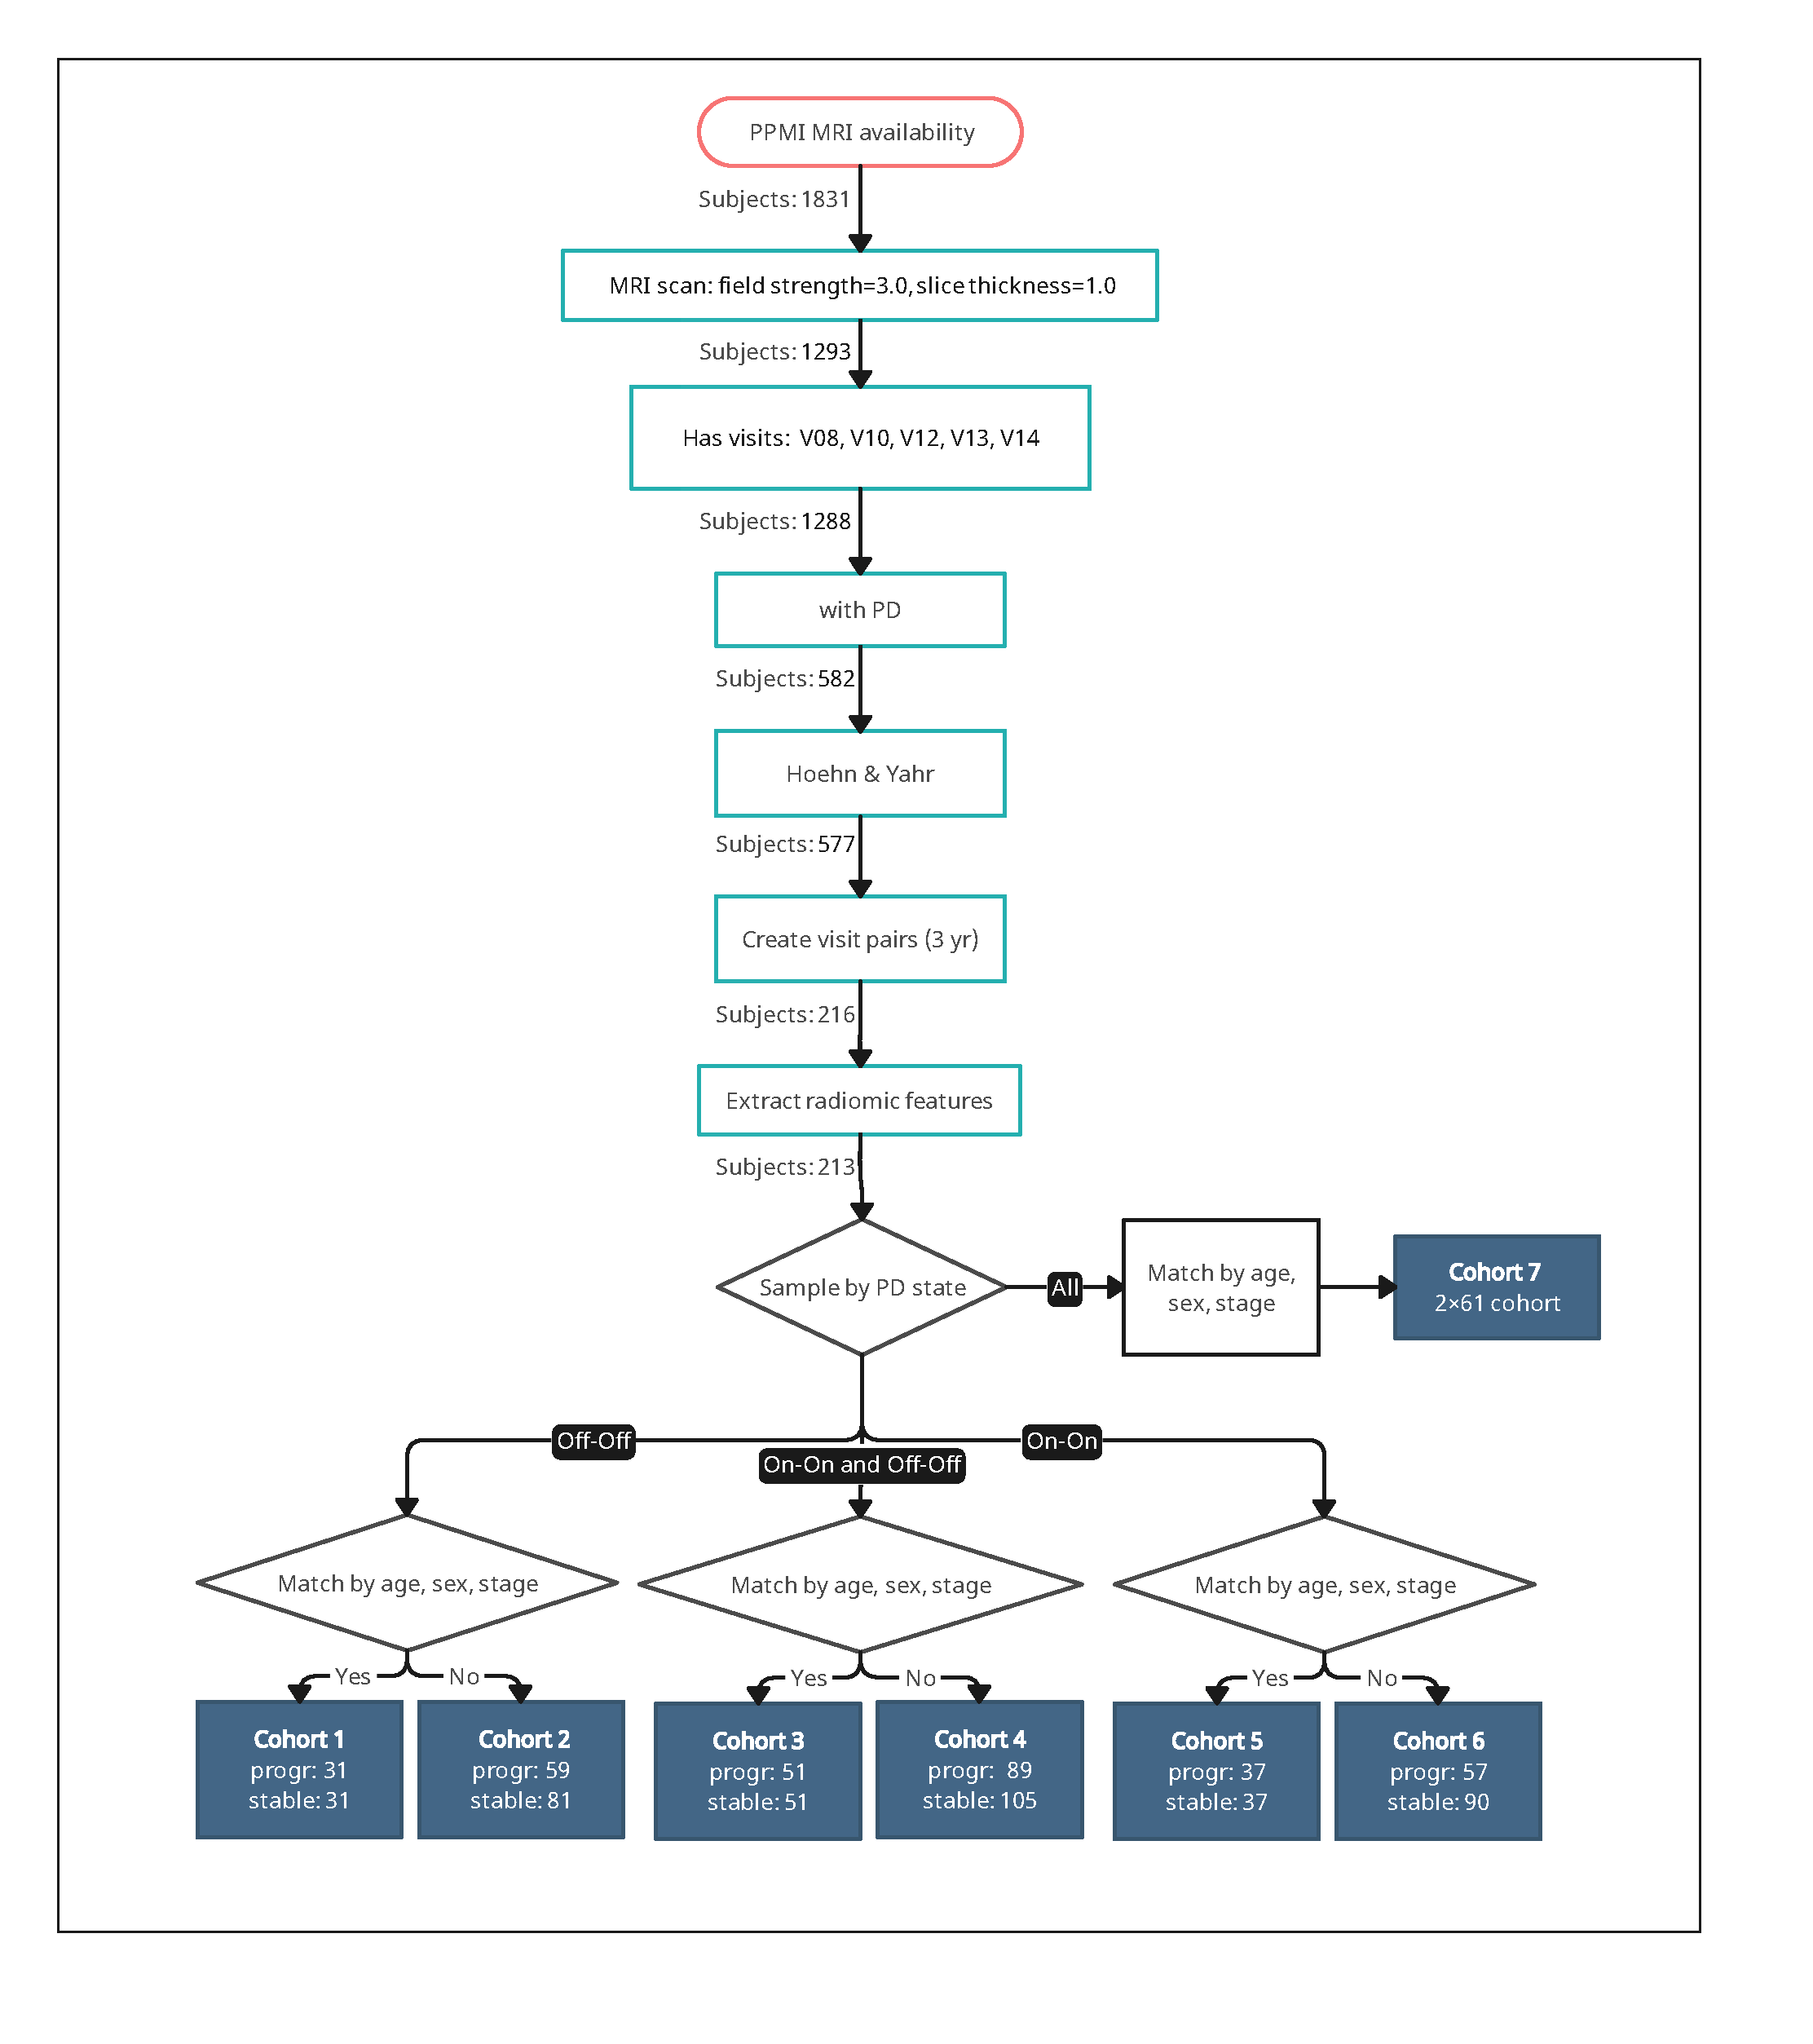
\includegraphics[width=\linewidth]{images/cohort_flowhart.pdf}
  \caption{{\bf Cohort construction} Process of filtering the PPMI dataset to construct 7 cohorts.}
  \label{cohortCreationFlowchart}
\end{figure}